\documentclass[12pt,a4paper]{article}

\usepackage[utf8]{inputenc}
\usepackage[T1]{fontenc}
\usepackage[english]{babel}
\usepackage{lmodern}
\usepackage{microtype}
\usepackage{amsmath}
\usepackage{amssymb}
\usepackage{geometry}
\usepackage{setspace}
\usepackage{booktabs}
\usepackage{array}
\usepackage{threeparttable}
\usepackage{adjustbox}
\usepackage{caption}
\usepackage{enumitem}
\usepackage{xcolor}
\usepackage{float}
\usepackage{graphicx}
\usepackage{tikz}
\usetikzlibrary{arrows.meta,positioning}
\usepackage{tabularray}
\usepackage{siunitx}
\usepackage[normalem]{ulem}
\UseTblrLibrary{booktabs}
\UseTblrLibrary{siunitx}
\newcommand{\tinytableTabularrayUnderline}[1]{\underline{#1}}
\newcommand{\tinytableTabularrayStrikeout}[1]{\sout{#1}}
\NewTableCommand{\tinytableDefineColor}[3]{\definecolor{#1}{#2}{#3}}
\usepackage[hidelinks]{hyperref}

\geometry{margin=1in}
\linespread{1.35}
\setlength{\parindent}{0.25in}
\setlength{\parskip}{0.25em}
\captionsetup{font=small,labelfont=bf}
\definecolor{linkblue}{RGB}{0,68,106}
\hypersetup{colorlinks=true,linkcolor=linkblue,citecolor=linkblue,urlcolor=linkblue}

\newcommand{\tabpath}{../3. Output/tables/}
\newcommand{\figpath}{../3. Output/figures/}
\newcommand{\sym}[1]{\ifmmode^{#1}\else\(^{#1}\)\fi}
\newcommand{\pp}{percentage points}

\title{The Decision to Hold Back: Teacher and Student Determinants of Grade Repetition}

\author{Ignacio Garijo-Campos \and Antonio Alfonso \and Pablo Bra\~nas-Garza \and Diego Jorrat \and Angel Sanchez}

\date{\today}

\begin{document}

\maketitle

\begin{abstract}
\noindent Grade repetition is a high-stakes educational decision, but most evidence studies its consequences for students rather than the teachers' decision process that produces it. We conduct a preregistered survey experiment with 2,705 teachers in Castilla-La Mancha, Spain. Teachers evaluate hypothetical student profiles and decide whether each student should repeat a grade. The experiment randomly varies whether teachers are exposed to policy alternatives, whether they rank those policies before assignment, and whether they are explicitly told if the assigned policy matches their preferences. The main result is that teacher and student characteristics explain repetition decisions much more than policy exposure or preference-policy alignment. Teachers respond strongly to student profiles: failed subjects increase repetition by 54.6 percentage points and low competence by 27.1 percentage points within teacher. Harsher teachers place especially large weight on failed subjects. Teacher characteristics and beliefs also matter. Secondary-school teachers, younger teachers, teachers with stronger meritocratic beliefs, and teachers who are more skeptical about resources for repeating students are harsher. In contrast, the preregistered treatment effects are small and mostly indistinguishable from zero. Sensitivity analyses using minimum detectable effects and equivalence tests show that the design can rule out several moderate effects but not all small alignment-specific effects. These results suggest that grade repetition is mainly driven by stable teacher profiles and by the academic information contained in student profiles, while light-touch policy assignment and alignment cues do not substantially alter repetition behavior.
\end{abstract}

\noindent\textbf{Keywords:} grade repetition; teacher decision-making; survey experiment; policy preferences; teacher beliefs.

\noindent\textbf{JEL codes:} I21; I24; C93; D91.

\section{Introduction}

\textcolor{red}{Grade repetition has been regarded as a double punishment for students, who not only face educational failure, but also have to deal with being segregated from their classmates. This can damage students' self-esteem and their perception of what they are capable of achieving. It can also increase costs for the education system and delay educational progression. Despite these concerns, grade repetition remains common in several education systems.}

\textcolor{red}{Spain is a particularly relevant setting. In PISA 2022, 22 percent of 15-year-old students in Spain reported having repeated a grade at least once, compared with an OECD average of 9 percent. This difference has made repetition an important education-policy issue. However, most research on grade repetition studies what happens to students after they repeat. Much less is known about the teacher-side decision process that generates repetition recommendations in the first place.}

\textcolor{red}{This paper shifts the perspective to teachers' decision-making. We conduct a preregistered survey experiment in Castilla-La Mancha, Spain, with 2,705 teachers. Teachers evaluate eight hypothetical students and decide whether each student should repeat a grade. Each student profile varies across six binary characteristics: gender, complex background, three or more failed subjects, low mathematical or linguistic competence, absenteeism, and disruptive behavior. This design allows us to estimate which student characteristics matter most for teachers when making repetition decisions.} It also allows us to estimate a teacher-level measure of \textit{harshness}, which we use to characterize harsher teachers.

The experiment also varies teachers' exposure to education policies. We can thus analyze how teachers react when they are assigned to different education policies, and if their decision-making regarding repetition is altered when the assigned policy is aligned with their preferences. The control group completes the repetition task freely, they are not assigned to an educational policy. In the treatment groups, teachers are randomly assigned to one of three policies before completing the repetition task. We present 3 variations of our treatment group, represented in table \ref{tab:design}. Policy treatment group is our baseline treatment group. They are assigned to a policy, then they complete the repetition task, and finally they rank the three policies from favorite to least favorite. The revelation treatment group ranks the policies first, so they have already revealed their preferences when they are randomly assigned to a policy. Finally, the awareness treatment follows the same path as the revelation treatment, but we prime them by reminding them if the policy they are assigned to is either their \textit{favorite}, \textit{least favorite}, or \textit{neither favorite nor least favorite}. This allows us to test whether policy exposure, preference revelation, and preference-policy alignment affect teacher harshness.

\textcolor{red}{Following the preregistered analysis plan, we construct several teacher-level harshness measures. The preferred measure compares each teacher's decisions with those of other teachers who saw the same student profile. We use this measure to characterize harsher teachers with both ordinary regressions and  random forest models}; and to test our pre-registered hypotheses on whether teacher's repetition decisions vary with policy exposure and alignment of assigned policies and their preferences.

Results show that repetition decisions are driven by teacher and student level characteristics, rather than assigned educational policies or  the alignment of said assignation with their preferences. 

Firstly, we see that younger teachers, that teach in secondary school, belief in effort rather than luck and show skepticism on resources dedicated to repeating students are associated with higher harshness levels.

Secondly, the random assignation of student characteristics suggest that teachers' decisions are mostly academically driven. A hypothetical student with three or more failed subjects is 54.6 p.p. more probable to be set to repeat. Showing low math/linguistic competence is also very relevant, and attitude-based characteristics like absenteeism and disruptive behavior also increase significantly the probability of repeating. Nonetheless, having a complex social background reduces it, and the gender of the student does not matter. Additionally, harsher teachers are even more academically driven, while lenient ones are comparatively more triggered by disruptive behavior and absenteeism.

Thirdly, education policies do not seem to affect retention decisions in any way. Teachers do not change their behavior when they are told to act under a specific policy. They also do not decide differently when they are assigned their favorite nor their least favorite policy. These results hold for all of our treatment groups, even when the assignation of the policy includes a priming message reminding them they have been assigned to their favorite or least favorite policy. However, their preferred education policy is always determinant for the level of harshness, which supports the results on teacher characterization which showed that variables related to ideology (belief in effort vs. luck and resource skepticism) were highly associated with harsher teachers.

All in all, our results suggest that, within our experiment, repetition decisions are defined by predetermined characteristics of teachers and students, rather than assigned educational policy or teacher's content with the policies they were assigned to.

\textcolor{red}{This paper is related to a growing literature on grade retention, teacher expectations, and teacher decision-making. It is not the first paper to use vignette or survey methods to study teachers' views about repetition. Recent and older work has studied teachers' beliefs about retention and the factors that enter retention judgments. Our contribution is narrower but, we think, important: to our knowledge, this is among the first preregistered survey experiments with teachers that jointly studies repetition decisions, random policy assignment, preference revelation, and explicit preference-policy alignment. This combination allows us to distinguish the determinants of repetition decisions from the effects of policy exposure itself.}

\section{Related literature}

The first related literature studies the effects of grade repetition on students. Repetition is often justified as a way to give students more time to acquire basic competencies, but empirical evidence is cautious. Some studies find short-run improvements in specific contexts, especially when retention is linked to remediation. Other studies find negative medium- or long-run effects on dropout and educational attainment. Alet, Bonnal, and Favard (2013) show that repetition in France produces short-run gains that become negative after several years. Cabrera-Hernandez (2022) studies a reform in Mexico and shows that reducing repetition lowered dropout without reducing average performance. OECD evidence also documents that systems with high repetition rates often do not perform better.

The second literature studies teacher expectations and teacher decisions. Teachers' expectations are consequential because they affect recommendations, grading, tracking, feedback, and student self-perception. This literature emphasizes that teacher judgments may combine valid information, professional experience, and bias. In the context of grade repetition, the relevant question is not simply whether teachers are biased, but which student characteristics they weight when deciding whether a student should repeat.

The third literature studies teachers' beliefs about grade retention. Tomchin and Impara (1992) show that teachers may view repetition as an acceptable practice even when research evidence is skeptical about its benefits. More recent vignette work also shows that academic performance, student behavior, gender, and teachers' own attitudes can affect retention decisions. This is directly connected to our design, because we experimentally vary student characteristics and observe teachers' decisions.

The fourth literature concerns policy exposure and motivated reasoning. Information and policy cues do not always translate into behavioral change, particularly when decisions are anchored in professional routines. In our setting, teachers may have stable views about repetition formed through classroom experience. A short policy assignment or an alignment reminder may therefore be too weak to change the decision rule.

\section{Experimental design and data}

\subsection{The repetition task}

Teachers complete a repetition task, also referred to in the preregistration as the card game. Each card represents a hypothetical student with six binary characteristics. The characteristics are: male/female, complex background/no, failed three or more subjects/no, low mathematical or linguistic abilities/no, serious disciplinary infraction/no, and frequent unjustified absenteeism/no. Teachers are asked whether the student should repeat the grade.

Before the task, teachers are shown two examples. One is an ideal student with no negative characteristics. The other is a student with all characteristics associated with grade repetition. These examples were included to make the task clear and to work as an attention check.

The analysis sample contains 2,705 teachers. Each teacher was asked to evaluate eight students. I do not report the average number of valid teacher-card decisions here because the preregistered design is based on eight cards per teacher and any discrepancy in valid counts should be audited separately.

\subsection{Teacher harshness}

The preregistration defines several measures of teacher harshness. We keep all of them in the analysis and report the alternatives in the appendix.


The preferred measure is the average deviation from other teachers who evaluated the same card. We define it in two steps. First, for each teacher-card decision, we compute the distance between teacher \(j\)'s decision for card \(i\) and the leave-one-out repetition rate for that same card:
\[
d_{ij}=R_{ij}-\bar{R}_{i,-j}.
\]
Here, \(R_{ij}\) equals one if teacher \(j\) recommends repetition for card \(i\), and zero otherwise. The term \(\bar{R}_{i,-j}\) is the average repetition rate for card \(i\) among all other teachers who evaluated that same card, excluding teacher \(j\). Second, we average those distances across the cards evaluated by teacher \(j\):
\[
H^b_j=\frac{1}{n_j}\sum_{i\in I_j} d_{ij}.
\]
A positive value means that the teacher is harsher than other teachers facing the same student profiles.

The third and fourth measures compare the teacher's decision with the predicted probability of repetition for the card. The prediction is obtained from a model using the six student characteristics, and in the more complete version also the education level and school ownership. These alternative measures are useful robustness checks because they adjust for profile difficulty in a parametric way.

\subsection{Treatment arms}

The experiment has four arms.


Table \ref{tab:design} recreates the preregistered conceptual map in a more formal format.

\begin{table}[H]
\centering
\caption{Experimental design}
\label{tab:design}
\begin{adjustbox}{max width=\textwidth}
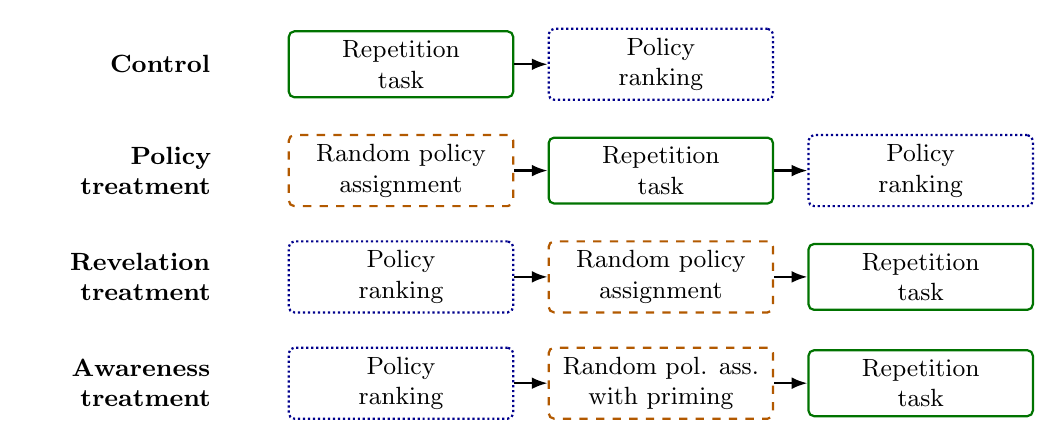
\begin{tikzpicture}[
  x=1cm, y=1cm,
  boxstep/.style={rounded corners=2pt, align=center, minimum width=2.85cm, minimum height=0.82cm, font=\small},
  taskstep/.style={boxstep, draw=green!45!black, thick},
  rankstep/.style={boxstep, draw=blue!55!black, densely dotted, thick},
  assignstep/.style={boxstep, draw=orange!70!black, dashed, thick},
  arm/.style={font=\small\bfseries, align=right, text width=2.2cm, anchor=east},
  arrow/.style={-{Latex[length=2mm]}, thick}
]
\node[arm] (c0) at (0,0) {Control};
\node[taskstep] (c1) at (2.3,0) {Repetition\\task};
\node[rankstep] (c2) at (5.6,0) {Policy\\ranking};
\draw[arrow] (c1) -- (c2);

\node[arm] (p0) at (0,-1.35) {Policy\\treatment};
\node[assignstep] (p1) at (2.3,-1.35) {Random policy\\assignment};
\node[taskstep] (p2) at (5.6,-1.35) {Repetition\\task};
\node[rankstep] (p3) at (8.9,-1.35) {Policy\\ranking};
\draw[arrow] (p1) -- (p2);
\draw[arrow] (p2) -- (p3);

\node[arm] (r0) at (0,-2.70) {Revelation\\treatment};
\node[rankstep] (r1) at (2.3,-2.70) {Policy\\ranking};
\node[assignstep] (r2) at (5.6,-2.70) {Random policy\\assignment};
\node[taskstep] (r3) at (8.9,-2.70) {Repetition\\task};
\draw[arrow] (r1) -- (r2);
\draw[arrow] (r2) -- (r3);

\node[arm] (a0) at (0,-4.05) {Awareness\\treatment};
\node[rankstep] (a1) at (2.3,-4.05) {Policy\\ranking};
\node[assignstep] (a2) at (5.6,-4.05) {Random pol. ass.\\with priming};
\node[taskstep] (a3) at (8.9,-4.05) {Repetition\\task};
\draw[arrow] (a1) -- (a2);
\draw[arrow] (a2) -- (a3);
\end{tikzpicture}
\end{adjustbox}
\begin{minipage}{0.92\textwidth}

\end{minipage}
\end{table}

\subsection{Preregistered hypotheses}

The preregistration expresses the hypotheses as null hypotheses. I keep that wording here because it helps interpret the results.

\textbf{H1\(|\)1.} Teachers' harshness is not correlated with being assigned to policies. This means that teachers assigned to the Policy treatment are not harder than those from the Control group.

\textbf{H1\(|\)2.} Teachers' harshness is not correlated with being assigned to a specific policy. This means that policy assignment has no impact on teachers' harshness.

\textbf{H1\(|\)3.} Teachers' harshness is not correlated with the alignment of teachers' preferences and their policy assignment. This means that teachers assigned to their favorite or least favorite policies are neither harder nor softer.

\textbf{H2\(|\)1.} Teachers' harshness is not correlated with being asked to rank the policies before policy assignment. This means that teachers assigned to the Revelation treatment are not harder than those from the Policy treatment.

\textbf{H2\(|\)2.} Teachers' harshness is not correlated with being assigned to a specific policy after having ranked the policies. This means that the interaction of treatment assignment and policy assignment has no impact on teachers' harshness.

\textbf{H2\(|\)3.} Teachers' harshness is not correlated with the alignment of teachers' preferences and their policy assignment when teachers have ranked the policies before assignment. This means that teachers assigned to their favorite or least favorite policies after having ranked them are neither harder nor softer than those who had not revealed them before the ranking.

\textbf{H3\(|\)1.} Teachers' harshness is not correlated with acknowledging their opinion of the policy they are being assigned to. This means that teachers assigned to the Awareness treatment are not harder than those from the Revelation treatment.

\textbf{H3\(|\)2.} Teachers' harshness is not correlated with being made aware of their opinions when assigning a specific policy. This means that the interaction of treatment assignment and policy allocation has no impact on teachers' harshness.

\textbf{H3\(|\)3.} Teachers' harshness is not correlated with the alignment of teachers' preferences and their policy assignment in a setting where they are aware of the alignment or disalignment. This means that teachers are neither harder nor softer when assigned to their favorite or least favorite policies with full awareness of their opinion on that policy.

\textbf{H4\(|\)1.} Current decisions are independent of previous decisions in the repetition task. We do not estimate this hypothesis because the analysis data do not contain a validated card-level response order. The numeric card identifiers are design labels rather than observed sequence positions.

\textbf{H4\(|\)2.} Policy preferences are orthogonal to policy assignment. This tests conformity in the Policy treatment.

\textbf{H4\(|\)3.} Treatment assignment has no effect on policy preferences.

\section{Empirical strategy}

The confirmatory analysis estimates ordinary least squares models using teacher harshness as the dependent variable. The outcome in the main tables is \(H^b_j\), the average deviation from other teachers seeing the same cards. Study I compares Control and Policy treatment. Study II compares Policy treatment and Revelation treatment. Study III compares Revelation treatment and Awareness treatment. Depending on the hypothesis, the regressions include treatment-arm indicators, assigned-policy indicators, favorite-policy indicators, and interactions between treatment arm and assigned policy.

The descriptive student-profile analysis uses the card-level decisions only to estimate the weight of student characteristics. To avoid confusing teacher harshness with attribute weights, we estimate linear probability models with teacher fixed effects. The model is:
\[
Y_{ij} =
\alpha_j +
\beta_1 X^{male}_{ij} + \beta_2 X^{background}_{ij} + \beta_3 X^{failed}_{ij}
+ \beta_4 X^{competence}_{ij} + \beta_5 X^{absent}_{ij}
+ \beta_6 X^{disruptive}_{ij} + \varepsilon_{ij}.
\]
The teacher fixed effect \(\alpha_j\) means that the coefficients are identified by comparing cards evaluated by the same teacher.
This model is descriptive. It answers which characteristics are associated with higher repetition probability within the same teacher.

For teacher characterization, we estimate both OLS regressions and random forest models. The OLS regressions are easy to interpret and imitate the preregistered covariate analysis.  The random forest models follow the preregistered plan, but we report them in the appendix because their role is diagnostic: they check whether the same broad teacher characteristics emerge when we use a more flexible predictive model. We also add the narrow resource-skepticism measure to both the OLS and random forest characterization.

\section{Descriptive results}

\subsection{Teacher characteristics and beliefs}

Table \ref{tab:characterization} characterizes harsher teachers using the preferred harshness measure. The first column includes the preregistered \(X_1\) covariates. The second column adds the \(X_2\) covariates from the second survey. The third column adds the narrow resource-skepticism index.

\begin{table}[H]
\centering
\caption{Teacher characteristics associated with harshness}
\label{tab:characterization}
\begin{adjustbox}{max width=\textwidth}
\input{\tabpath paper_rewrite_characterization_regression.tex}
\end{adjustbox}
\end{table}

Several patterns are stable. Secondary-school teachers are harsher than primary-school teachers. Age is negatively associated with harshness: younger teachers are harsher. Belief in effort is positively associated with harshness. Most importantly for the belief analysis, resource skepticism is strongly associated with harshness. A one standard deviation increase in resource skepticism predicts a 2.1 percentage point increase in relative harshness in the characterization regression.

This resource-skepticism index is intentionally narrow. It uses two items: whether too many resources are allocated to repeating students, and whether additional resources for repeating students are ineffective. We do not use the broader belief index in the main paper because it combines too many different concepts and has low internal consistency. The narrow index is more homogeneous and easier to interpret.


Appendix Table \ref{tab:rf_importance} reports the random forest characterization. The results are broadly consistent with the regression evidence in highlighting teacher characteristics and beliefs as relevant predictors, but the random forest should be read as a descriptive predictive exercise rather than as an inferential ranking of individual coefficients.

\subsection{Student characteristics in the repetition task}

Table \ref{tab:attributes} reports the only card-level analysis kept in the main text. The purpose is descriptive: it tells the reader which student characteristics teachers use when deciding repetition.

\begin{table}[H]
\centering
\caption{Descriptive within-teacher weights of student characteristics}
\label{tab:attributes}
\input{\tabpath paper_rewrite_attribute_weights.tex}
\begin{minipage}{0.92\textwidth}
\footnotesize \textit{Notes:} The model includes teacher fixed effects. Standard errors are clustered by teacher. Coefficients are probability-point effects.
\end{minipage}
\end{table}

The result is clear. Failed subjects dominate the decision. Holding the other student characteristics constant and comparing cards within the same teacher, having three or more failed subjects increases repetition by 54.6 \pp. Low competence increases repetition by 27.1 \pp. Absenteeism and disruptive behavior matter, but much less. Male gender does not matter. Complex background has a negative coefficient once the other attributes are held constant.

Table \ref{tab:attributes_harshness} shows the same descriptive model by terciles of teacher harshness. This makes the heterogeneity easy to communicate. Harsher teachers place especially high weight on failed subjects. In the lenient tercile, failed subjects increase repetition by 33.2 \pp. In the middle and harsh terciles, the effect is about 65 \pp. By contrast, absenteeism and disruptive behavior are not what makes harsh teachers harsher. In the harsh tercile, the coefficient on absenteeism is close to zero and the coefficient on disruptive behavior is negative conditional on the other characteristics. This does not mean that harsh teachers reward disruption. It means that their additional harshness is concentrated in academic failure signals, especially failed subjects.

\begin{table}[H]
\centering
\caption{Student-characteristic weights by teacher harshness tercile}
\label{tab:attributes_harshness}
\input{\tabpath paper_rewrite_attribute_weights_by_harshness.tex}
\begin{minipage}{0.92\textwidth}
\footnotesize \textit{Notes:} Each column estimates the within-teacher descriptive model separately for teachers in the corresponding tercile of the preferred harshness measure. Coefficients are probability-point effects. Stars indicate significance: * \(p<0.1\), ** \(p<0.05\), *** \(p<0.01\).
\end{minipage}
\end{table}

\section{Preregistered results}

\subsection{Study I: Policy treatment vs. Control}

Study I compares teachers in the Control group with teachers in the Policy treatment.

H1\(|\)1 states that teachers' harshness is not correlated with being assigned to policies. The estimate in Table \ref{tab:h1} is small and not significant. Teachers in the Policy treatment are not harsher than teachers in the Control group.

H1\(|\)2 states that teachers' harshness is not correlated with being assigned to a specific policy. The assigned-policy coefficients are not statistically significant. This suggests that being assigned to reinforcement, modified promotion criteria, or teacher training does not meaningfully change harshness relative to Control.

\begin{table}[H]
\centering
\caption{Study I: H1\(|\)1 and H1\(|\)2}
\label{tab:h1}
\begin{adjustbox}{max width=\textwidth}
\input{\tabpath paper_rewrite_h1_agg.tex}
\end{adjustbox}
\end{table}

H1\(|\)3 states that teachers' harshness is not correlated with the alignment between their preferences and their policy assignment. Table \ref{tab:h13} restricts the sample to Control teachers and treated teachers assigned to either their favorite or least favorite policy. Neither favorite assignment nor least-favorite assignment significantly changes harshness.

\begin{table}[H]
\centering
\caption{Study I: H1\(|\)3}
\label{tab:h13}
\begin{adjustbox}{max width=\textwidth}
\input{\tabpath paper_rewrite_h13.tex}
\end{adjustbox}
\end{table}

\subsection{Study II: Revelation treatment vs. Policy treatment}

Study II compares the Revelation treatment with the Policy treatment. The difference is that teachers in Revelation rank policies before policy assignment.

H2\(|\)1 states that teachers' harshness is not correlated with being asked to rank the policies before policy assignment. Table \ref{tab:h2} shows no significant difference between Revelation and Policy treatment.

H2\(|\)2 states that teachers' harshness is not correlated with being assigned to a specific policy after having ranked the policies. The interacted model in Table \ref{tab:h2} does not show a broad pattern of treatment-policy effects. The contrast table, Table \ref{tab:h22}, shows one suggestive result: for Policy 2, Revelation teachers are harsher than Policy-treatment teachers assigned to the same policy. This estimate is significant at the 10 percent level. Since it is one contrast among several and does not survive a more conservative reading, it should be treated as suggestive rather than central.

\begin{table}[H]
\centering
\caption{Study II: H2\(|\)1 and H2\(|\)2}
\label{tab:h2}
\begin{adjustbox}{max width=\textwidth}
\input{\tabpath paper_rewrite_h2_agg.tex}
\end{adjustbox}
\end{table}

\begin{table}[H]
\centering
\caption{Study II: H2\(|\)2 contrasts by assigned policy}
\label{tab:h22}
\input{\tabpath paper_rewrite_h22_contrasts.tex}
\end{table}

H2\(|\)3 states that teachers' harshness is not correlated with preference-policy alignment when preferences have been ranked before assignment. Table \ref{tab:h23} estimates separate regressions for teachers assigned to their favorite policy and teachers assigned to their least favorite policy. The Revelation coefficient is not significant in either subsample.

\begin{table}[H]
\centering
\caption{Study II: H2\(|\)3}
\label{tab:h23}
\begin{adjustbox}{max width=\textwidth}
\input{\tabpath paper_rewrite_h23.tex}
\end{adjustbox}
\end{table}

\subsection{Study III: Awareness treatment vs. Revelation treatment}

Study III compares Awareness treatment with Revelation treatment. The difference is that Awareness teachers are explicitly told whether the assigned policy is their favorite, neither favorite nor least favorite, or least favorite policy.

H3\(|\)1 states that teachers' harshness is not correlated with acknowledging their opinion of the policy they are assigned to. Table \ref{tab:h3} shows that Awareness teachers are not significantly harsher than Revelation teachers.

H3\(|\)2 states that teachers' harshness is not correlated with being made aware of their opinions when assigning a specific policy. The interacted model does not show significant treatment-policy effects. The contrast table, Table \ref{tab:h32}, also shows no meaningful differences by assigned policy.

\begin{table}[H]
\centering
\caption{Study III: H3\(|\)1 and H3\(|\)2}
\label{tab:h3}
\begin{adjustbox}{max width=\textwidth}
\input{\tabpath paper_rewrite_h3_agg.tex}
\end{adjustbox}
\end{table}

\begin{table}[H]
\centering
\caption{Study III: H3\(|\)2 contrasts by assigned policy}
\label{tab:h32}
\input{\tabpath paper_rewrite_h32_contrasts.tex}
\end{table}

H3\(|\)3 states that teachers' harshness is not correlated with preference-policy alignment in a setting where they are aware of the alignment or disalignment. Table \ref{tab:h33} shows no significant effect for teachers assigned to their favorite policy or to their least favorite policy.

\begin{table}[H]
\centering
\caption{Study III: H3\(|\)3}
\label{tab:h33}
\begin{adjustbox}{max width=\textwidth}
\input{\tabpath paper_rewrite_h33.tex}
\end{adjustbox}
\end{table}

\subsection{Study IV: additional preregistered analyses}

H4\(|\)1 is not estimated because the analysis data do not contain a validated sequence of card decisions. This is an important limitation. The preregistered test concerns whether current decisions depend on previous decisions, but the available card identifiers should not be interpreted as response order.

H4\(|\)2 asks whether policy preferences are orthogonal to policy assignment in the Policy treatment. Appendix Table \ref{tab:h42} reports logit models for whether being assigned to a policy predicts later ranking it as favorite or least favorite.

H4\(|\)3 asks whether treatment assignment affects policy preferences. Appendix Table \ref{tab:h43} reports the share of teachers ranking each policy as favorite or least favorite by treatment arm, with confidence intervals.

\section{Sensitivity analyses: MDE and equivalence tests}

Because many preregistered estimates are null, we add two sensitivity analyses. The first is the minimum detectable effect with 80 percent power. This tells us which effect sizes the design was able to detect with reasonable probability. The second is an equivalence test. This asks whether we can reject effects outside a given substantive margin.

These tests should not replace the preregistered hypotheses. They help interpret them. For broad treatment-arm contrasts, the MDEs are around 2.7 to 3.8 \pp. The equivalence tests show that H1\(|\)1, H2\(|\)1, and H3\(|\)1 are equivalent to zero under a 3 \pp margin. This means that moderate average treatment effects can be ruled out for the main treatment comparisons.

The evidence is weaker for the more granular policy-assignment and alignment hypotheses. Many of those estimates are not equivalent to zero under a 3 \pp margin. This does not mean they are significant; it means that the design cannot rule out small effects for every policy-specific or alignment-specific contrast. This distinction is important. The paper should state that the policy and alignment estimates are mostly null, while also acknowledging that some granular effects are imprecisely estimated.

\section{Discussion}

The results point to a simple but important conclusion. Grade repetition decisions are mostly explained by the teachers who make them and the student profiles they evaluate. Policy exposure and preference-policy alignment do not substantially alter repetition behavior.

The descriptive card-level results show that teachers respond strongly to academic information. Failed subjects are by far the strongest predictor of repetition. Low competence also matters substantially. Behavioral indicators matter less. This suggests that repetition decisions are structured around academic failure rather than around a general negative evaluation of the student.

The teacher-characterization results show that harshness is also related to teacher profiles and beliefs. Secondary-school teachers are harsher, younger teachers are harsher, and teachers with stronger beliefs in effort and resource skepticism are harsher. These patterns are not causal, but they are informative for policy. If policymakers want to understand why repetition remains common, it is not enough to look at policy rules. They also need to understand the professional beliefs and contexts that shape teachers' thresholds.

The preregistered treatment results are mostly null. Teachers do not become substantially harsher or softer when exposed to policy alternatives, when they reveal preferences before assignment, or when they are made aware that the assigned policy matches or conflicts with their preferences. This is particularly relevant for the alignment hypotheses. The experiment was designed to test whether teachers might respond differently when they feel heard or ignored. We find little evidence that this mechanism changes repetition decisions.

The paper therefore should not be framed as a story in which preferences move but behavior does not. That may be an interesting secondary observation, but it is not the main contribution. The stronger contribution is that student characteristics and teacher characteristics explain repetition decisions, while policies and alignment do not appear to alter them much.

\section{Conclusion}

This paper studies teacher decision-making in grade repetition using a preregistered survey experiment with 2,705 teachers. Teachers evaluated hypothetical student profiles and were randomly assigned to policy environments that varied policy exposure, preference revelation, and awareness of preference-policy alignment.

The main finding is that repetition decisions are stable with respect to these policy manipulations. The preregistered treatment effects are generally small and statistically insignificant. Sensitivity analyses rule out several moderate average effects, although not all small granular effects. At the same time, repetition decisions are far from random. Teachers respond strongly to student characteristics, especially failed subjects and low competence. Harsher teachers place particularly strong weight on failed subjects. Teacher characteristics and beliefs, including resource skepticism, are associated with higher harshness.

The policy implication is that light-touch exposure to policies or alignment messages is unlikely to change repetition behavior on its own. If policymakers aim to reduce unnecessary repetition, they may need to focus on decision protocols, credible remediation alternatives, and the beliefs that shape teachers' thresholds for repetition.

\clearpage
\appendix

\section{Alternative harshness measures}


The preregistration proposed several harshness measures. The first is the share of repetitions recommended by teacher \(j\):
\[
H^a_j=\frac{1}{n_j}\sum_{i\in I_j} R_{ij}.
\]
This measure is intuitive, but it does not adjust for the fact that some teachers may see harder cards. The second measure is the preferred leave-one-out deviation measure used in the main analysis:
\[
d_{ij}=R_{ij}-\bar{R}_{i,-j}, \qquad H^b_j=\frac{1}{n_j}\sum_{i\in I_j}d_{ij}.
\]
The third measure replaces the leave-one-out card average with a predicted probability from a logit model using the six student characteristics:
\[
H^c_j=\frac{1}{n_j}\sum_{i\in I_j}(R_{ij}-\widehat{R}_i).
\]
The fourth measure uses the same logic but obtains \(\widehat{R}^{\,c}_i\) from a more complete prediction model that also includes teacher education level and school ownership:
\[
H^d_j=\frac{1}{n_j}\sum_{i\in I_j}(R_{ij}-\widehat{R}^{\,c}_i).
\]
Table \ref{tab:appendix_harshness} repeats the characterization regression using these four outcomes.

\begin{table}[H]
\centering
\caption{Teacher characterization using alternative harshness measures}
\label{tab:appendix_harshness}
\begin{adjustbox}{max width=\textwidth}
\input{\tabpath paper_rewrite_harshness_measures_appendix.tex}
\end{adjustbox}
\end{table}

\section{Random forest characterization}

The random forest analysis follows the preregistered idea of using flexible predictive models to characterize harsher teachers. We report it in the appendix because the OLS characterization is easier to interpret in the main text. Table \ref{tab:rf_importance} reports permutation importance across repeated forests. This is not a causal ranking and should not be read as a substitute for the regression coefficients. Its purpose is more limited: to check whether a flexible predictive model points to a similar set of teacher characteristics.

\begin{table}[H]
\centering
\caption{Random forest permutation importance for teacher harshness}
\label{tab:rf_importance}
\begin{adjustbox}{max width=\textwidth}
\input{\tabpath paper_rewrite_rf_importance.tex}
\end{adjustbox}
\begin{minipage}{0.92\textwidth}
\footnotesize \textit{Notes:} The table reports mean permutation importance across 50 random forests. Intervals summarize variation across repeated forests and should be interpreted as stability intervals, not causal confidence intervals.
\end{minipage}
\end{table}

\begin{figure}[H]
\centering
\caption{Harshness and significant teacher characteristics}
\label{fig:harshness_correlations}
\includegraphics[width=\textwidth]{\figpath paper_rewrite_harshness_significant_predictors.jpeg}
\begin{minipage}{0.92\textwidth}
\footnotesize \textit{Notes:} The figure plots the bivariate relationship between the preferred harshness measure and the variables that are statistically significant in the main characterization regression: education level, age, belief in effort, and resource skepticism. The panels are descriptive and do not replace the multivariate estimates in Table \ref{tab:characterization}.
\end{minipage}
\end{figure}

\section{MDE and equivalence tests}

Table \ref{tab:mde} reports the minimum detectable effects for the preregistered teacher-level hypotheses. Table \ref{tab:equivalence} reports equivalence tests using a 3 percentage point margin. The script also exports the same equivalence analysis using 2 and 5 percentage point margins.

\begin{table}[H]
\centering
\caption{Minimum detectable effects for preregistered teacher-level hypotheses}
\label{tab:mde}
\begin{adjustbox}{max width=\textwidth}
\input{\tabpath paper_rewrite_teacher_mde.tex}
\end{adjustbox}
\end{table}

\begin{table}[H]
\centering
\caption{Equivalence tests for preregistered teacher-level hypotheses, 3 percentage point margin}
\label{tab:equivalence}
\begin{adjustbox}{max width=\textwidth}
\input{\tabpath paper_rewrite_teacher_equivalence.tex}
\end{adjustbox}
\end{table}

\section{Additional preregistered analyses}

\begin{table}[H]
\centering
\caption{H4\(|\)2: Policy assignment and later policy preferences}
\label{tab:h42}
\begin{adjustbox}{max width=\textwidth}
\input{\tabpath paper_rewrite_h42.tex}
\end{adjustbox}
\end{table}

\begin{table}[H]
\centering
\caption{H4\(|\)3: Policy preferences by treatment arm}
\label{tab:h43}
\begin{adjustbox}{max width=\textwidth}
\input{\tabpath paper_rewrite_h43_preference_shares.tex}
\end{adjustbox}
\end{table}

\section{Policies}

The experiment randomly assigned treated teachers to one of the following three policies, as described in the preregistration:

\begin{itemize}
\item \textbf{Policy A: Educational reinforcement.} The student will receive educational reinforcement in a small group next school year, with a support teacher, inside or outside the classroom.
\item \textbf{Policy B: Modified promotion criteria.} The promotion criteria will be modified in the Evaluation Board: unanimity for grade retention, secret and anonymous voting.
\item \textbf{Policy C: Teacher training.} All school staff will receive tailored training and teaching support in inclusive teaching methodologies and multi-level classroom management.
\end{itemize}

\section{Card-level robustness checks}

The main text keeps only the descriptive card-level attribute analysis. Additional card-level models, including treatment-by-attribute checks and belief-by-attribute checks, are generated by \texttt{2. Code/4. decision\_card\_models.R} and should be read as robustness or exploratory appendix material rather than as central results.

\begin{thebibliography}{99}

\bibitem{alet2013} Alet, E., Bonnal, L., and Favard, P. (2013). Repetition: Medicine for a short-run remission. \textit{Annals of Economics and Statistics}, 111/112, 227--250.

\bibitem{allen2009} Allen, C. S., Chen, Q., Willson, V. L., and Hughes, J. N. (2009). Quality of research design moderates effects of grade retention on achievement: A meta-analytic, multilevel analysis. \textit{Educational Evaluation and Policy Analysis}, 31(4), 480--499.

\bibitem{bonvin2003} Bonvin, P. (2003). The role of teacher attitudes and judgement in decision-making: The case of grade retention. \textit{European Educational Research Journal}, 2(2), 277--294.

\bibitem{cabrera2022} Cabrera-Hernandez, F. (2022). Leave them kids alone! The effects of abolishing grade repetition: Evidence from a nationwide reform. \textit{Education Economics}, 30(4), 339--355.

\bibitem{jacob2004} Jacob, B. A., and Lefgren, L. (2004). Remedial education and student achievement: A regression-discontinuity analysis. \textit{Review of Economics and Statistics}, 86(1), 226--244.

\bibitem{manacorda2012} Manacorda, M. (2012). The cost of grade retention. \textit{Review of Economics and Statistics}, 94(2), 596--606.

\bibitem{oecd2023} OECD (2023). \textit{PISA 2022 Results}. OECD Publishing.

\bibitem{tomchin1992} Tomchin, E. M., and Impara, J. C. (1992). Unraveling teachers' beliefs about grade retention. \textit{American Educational Research Journal}, 29(1), 199--223.

\end{thebibliography}

\end{document}
